\lab{Algorithms}{Modified Gram-Schmidt (QR)}{QR decomposition}
\label{lab:QRdecomp}
\objective{Use the Gram-Schmidt algorithm and orthonormal transformations to perform the QR decomposition.}

The QR decomposition of a matrix $A$ is a factorization $A=QR$, where $Q$ has orthonormal columns and $R$ is upper triangular.
This decomposition is useful for computing least squares and finding eigenvalues.
As stated in the following theorem, the QR decomposition of $A$ always exists when the rank of $A$ equals the number of columns of $A$.
\begin{theorem}
Let $A$ be an $m\times n$ matrix of rank $n$.  Then $A$ can be
factored into a product $Q R$, where $Q$ is an $m\times n$ matrix
with orthonormal columns and $R$ is a nonsingular $n \times n$ upper
triangular matrix.
\end{theorem}

\section*{Computing the QR Decomposition}
Let $A$ be an $m \times n$ matrix of rank $n$.
There are many methods for computing the QR decomposition.
First we will discuss the algorithm that computes $Q$ by applying Gram-Schmidt to the columns of $A$.

Let $\{\x_i\}_{i=1}^n$ be the columns of $A$ (the rank hypothesis implies that these are linearly independent vectors).
Then the Gram-Schmidt algorithm computes an orthonormal basis $\{\q_i\}_{i=1}^n$ for the span of the $\x_i$. 
The Gram-Schmidt algorithm defines  \[ \q_1 = \frac{\x_1}{\norm{\x_1}}.\]
It recursively defines $\q_k$ for $k>1$ by
\[
\q_{k} = \frac{\x_k - \p_{k-1}}{\|\x_k - \p_{k-1}\|}, \,\,\,\, k=2,\ldots,n,
\]
where
\[
\p_{k-1} = \sum_{i=1}^{k-1} \langle \q_i, \x_k\rangle \q_i, \,\,\,\, k=2, \ldots, n
\]
and $\p_0 = 0$. 

In the QR factorization of $A$, the matrix $Q$ has columns $\{\q_i\}_{i=1}^n$. The matrix $R$ is then the upper triangular matrix with entries $r_{jk}$ where $r_{kk} = \|\x_k-\p_{k-1}\|$ and $r_{j k} = \langle \q_j, \x_k\rangle$ when $j < k$. See [TODO: ref textbook] for a proof that $QR=A$ and $R$ is nonsingular.


When implemented with a computer, the Gram-Schmidt algorithm may produce a matrix $Q$ that is not even close to orthonormal due to rounding errors. We now introduce the modified Gram-Schmidt algorithm, which consistently produces matrices $Q$ that are ``very close'' to orthonormal.

In the modified Gram-Schmidt algorithm, $\q_1$ is the normalization of $\x_1$ as before. We then make each of the vectors $\x_2, \ldots, \x_n$ orthogonal to $\q_1$ by defining
\[
\x_k := \x_k - \langle \q_1,\x_{k} \rangle \q_1,\quad k=2,\ldots,n.
\]
(Compare this to the usual Gram-Schmidt algorithm, where we only made $\x_2$ orthogonal to $\q_1$.) Next we define $\q_2 = \frac{\x_2}{\|\x_2\|}.$ Once again we make $\x_3, \ldots, \x_n$ orthogonal to $\q_2$ by defining
\[
\x_k := \x_k - \langle \q_2,\x_{k} \rangle \q_2,\quad k=3,\ldots,n.
\]
(Each of these new vectors is a linear combination of vectors orthogonal to $\q_1$, and hence is orthogonal to $\q_1$ as well.) We continue this process until we have an orthonormal set $q_1, \ldots, q_k$. To summarize, the modified Gram-Schmidt algorithm is as follows.

%TODO: proofread this, explain notation, and make the LU decomposition alg. like this
\begin{algorithm}
\caption{Modified Gram-Schmidt}
\label{Alg:MGS}
\begin{algorithmic}[1]
\Procedure{Modified Gram-Schmidt}{$A$}
\State $m, n \gets \text{shape} \left( A \right)$
\State $Q \gets \text{copy} \left( A \right)$
\State $Q \gets \text{zeros}((n,n))$
\For{$0 \leq i < n$}
    \State $R_{i,i} \gets \norm{Q_{:,i}}$
    \State $Q_{:,i} \gets Q_{:,i}/R_{i,i}$
    \For{$i+1 \leq j < n$}
        \State $R_{i,j} \gets Q_{:,j}Q_{:,i}$
        \State $Q_{:,j} \gets Q_{:,j}-R_{i,j}Q_{:,i}$
	\EndFor
\EndFor
\State \pseudoli{return} $Q, R$
\EndProcedure
\end{algorithmic}
\end{algorithm}


\begin{problem}
\label{prob:QR}
Write your own implementation of the QR decomposition. Write a function \li{QR} that accepts as input a square matrix $A$ of full rank, and computes the QR decomposition, returning the matrices $Q$ and $R$ (which should be the same shape as $A$). Be sure to use the numerically stable Modified Gram-Schmidt algorithm. Also assume there are no zeros on the main diagonal.

You can test that you have the right decomposition by verifying that $QR=A$ and $Q^T Q = I$. While this is true most of the time, it may not always be true due to roundoff.
\end{problem}

\begin{problem}
The QR decomposition gives a really nice way to calculate the magnitude of the determinant of a square matrix of full rank. Write a function \li{QRDet} that accepts a square matrix of full rank as input, and returns the magnitude of the determinant of that matrix. Use your QR decomposition to perform this
calculation.

You may check your work by comparing your results to those produced by \li{scipy.linalg.det}. 
\end{problem}

%TODO: put this section after the next? What algorithm does SciPy use?
\section*{QR Decomposition in SciPy}
The linear algebra library in SciPy calculates the QR decomposition using a software package called LAPACK (Linear Algebra PACKage), which is incredibly efficient.
Here is an example of using SciPy to compute the QR decomposition of a matrix.

\begin{lstlisting}
>>> import numpy as np
>>> from scipy import linalg as la

>>> A = np.random.rand(4,3)
>>> Q, R = la.qr(A)
>>> Q.dot(R) == A                      
array([[ True, False, False],
       [ True, False, False],
       [ True,  True, False],
       [ True,  True, False]], dtype=bool)
\end{lstlisting}
 Note that \li{Q.dot(R)} does not equal \li{A} exactly because of rounding errors. However, we can check that the entries of \li{Q.dot(R)} are ``close'' to the entries of \li{A} with the NumPy method \li{np.allclose()}. This method checks that the elements of two arrays differ by less than a given tolerance, a tolerance specified by two keyword arguments \li{rtol} and \li{atol} that default to $10^{-5}$ and $10^{-8}$ respectively.
\begin{lstlisting}
>>> np.allclose(Q.dot(R), A) 
True
\end{lstlisting}
We can use the same method to check that \li{Q} is ``very close'' to an orthogonal matrix.
\begin{lstlisting}
>>> np.allclose(Q.T.dot(Q), np.eye(4)) 
True
\end{lstlisting}


\section*{Orthonormal transformations}
Another way to compute the QR decomposition of a matrix is with a series of orthonormal transformation. Like the Modified Gram-Schmidt algorithm, orthonormal transformations are numerically stable, meaning that they are less susceptible to rounding errors.\footnote{In lab [TODO: ref] we will define the \emph{condition number} of a matrix, which tells us about the numerical stability of the corresponding operator. Small condition numbers mean the operator is more stable. In fact, orthonormal matrices have the smallest possible condition number, which is 1.}

%TODO: revise this section
\section*{Householder reflections}
A Householder reflection is a linear transformation $P: \mathbb{R}^n \rightarrow \mathbb{R}^n$ that reflects a vector $x$ about a hyperplane.
See figure \ref{fig:Householder_reflector}.
Recall that a hyperplane can be defined by a unit vector $v$ which is orthogonal to the hyperplane. 
As shown in figure \ref{fig:Householder_reflector}, $x - \langle v,x \rangle v$ is the projection of $x$ onto the hyperplane orthogonal to $v$.
However, to reflect \emph{across} the hyperplane, we must move twice as far; that is, $Px = x - 2\langle v,x \rangle v$.
This can be written $Px = x - 2v(v^\mathsf{H} x)$, so $P$ has matrix representation $P = I - 2v v^\mathsf{H}$.
Note that $P^\mathsf{H} P = I$; thus $P$ is orthonormal.

\begin{figure}
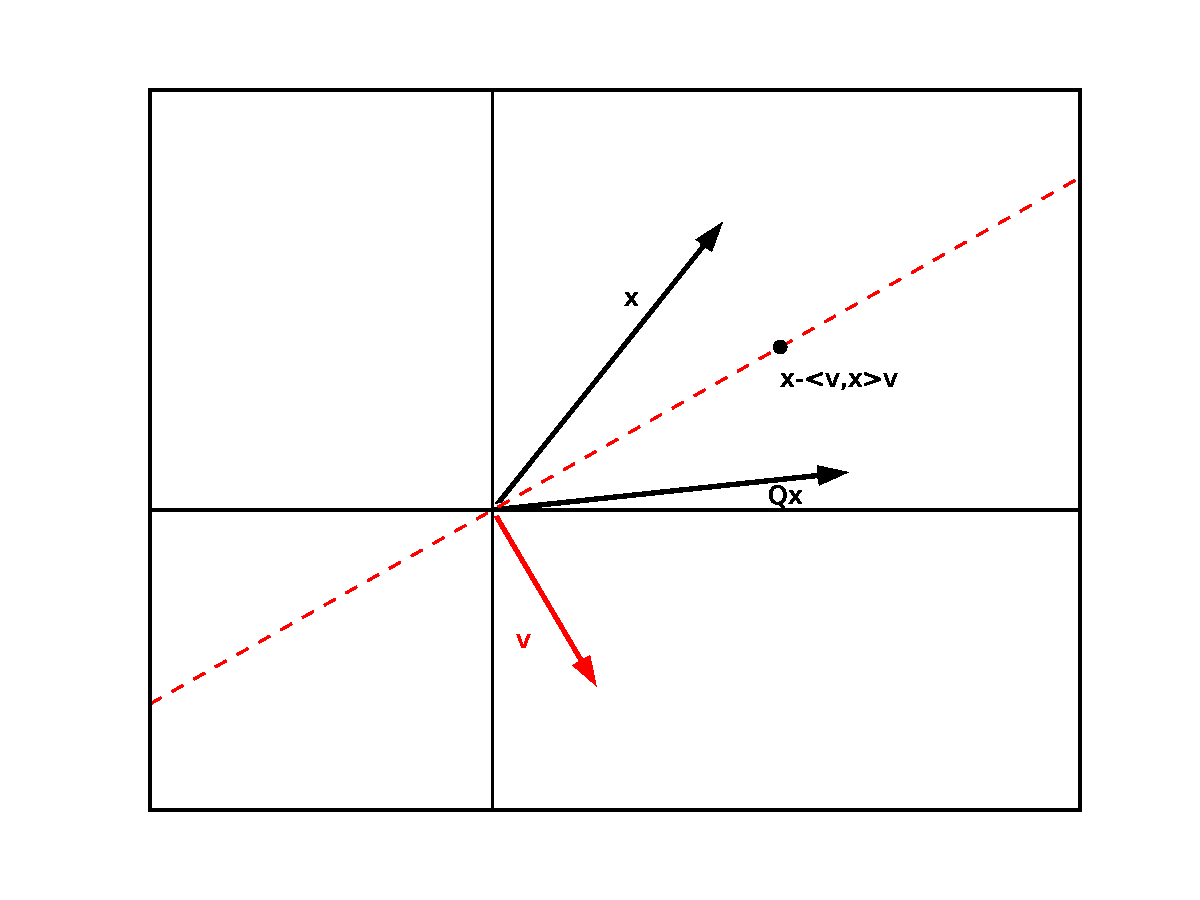
\includegraphics[width= \textwidth]{fig1}
\caption{Householder reflector}
\label{fig:Householder_reflector}
\end{figure}

\subsection*{Householder triangularization}
The QR decomposition of an $m \times n$ matrix $A$ can also be computed with Householder transformations via the Householder triangularization.
Whereas Gram-Schmidt makes $A$ \emph{orthonormal} using a series of transformations stored in an \emph{upper triangular} matrix, Householder triangularization makes $A$ \emph{triangular} by a series of \emph{orthonormal} transformations.
More precisely, the Householder triangularization finds an $m \times m$ orthogonal matrix $Q$ and and $m \times n$ upper triangular matrix $R$ such that $QA = R$. 
Since $Q$ is orthogonal, $Q^{-1}=Q^T$ so $A = QR$.
(Contrast this with the QR decomposition where $A = QR$, the matrix $Q$ is $m \times n$, and $R$ is $n \times n$). 
If $A$ is square, then $A = Q^TR$ is the QR decomposition. 

Let's demonstrate the idea behind Householder triangularization on a $4 \times 3$ matrix $A$.
Let $e_1, \ldots, e_4$ be the standard basis of $\mathbb{R}^4$.
First we find an orthonormal transformation $Q_1$ that maps the first column of A into the span of $e_1$. This is diagrammed below, where and $*$ represents an arbitrary entry.

\def\mc#1{\multicolumn{1}{c|}{#1}}
\def\lc#1{\multicolumn{1}{|c}{#1}}
\begin{equation*}
\begin{pmatrix}
* & * & * \\
* & * & * \\
* & * & * \\
* & * & *
\end{pmatrix}
\underrightarrow{Q_1}
\begin{pmatrix}

* & * & * & \\ \cline{2-3}
\mc{0} & * & \mc{*}& \\
\mc{0} & * & \mc{*} & \\
\mc{0}& * & \mc{*} & \\ \cline{2-3}
\end{pmatrix}
\end{equation*}
Let $A_2 = Q_1A$ be the matrix on the right above.
Now find an orthonormal transformation $Q_2$ that fixes $e_1$ and maps the second column of $A_2$ into the span of $e_1$ and $e_2$. Notice that since $Q_2$ fixes $e_1$, the top row of $A_2$ will be fixed by $Q_2$, and only entries in the boxed submatrix will change.

%\def\mc#1{\multicolumn{1}{c|}{#1}}
%\begin{equation*}
%\begin{pmatrix}
%* & * & * & \\ \cline{2-3}
%\mc{0} & * & \mc{*}& \\
%\mc{0} & * & \mc{*} & \\
%\mc{0}& * & \mc{*} & \\ \cline{2-3}
%\end{pmatrix}
%
%\underrightarrow{Q_1}
%
%\begin{pmatrix}
%* & * & * & \\ \cline{2-3}
%\mc{0} & 0 & \mc{*}& \\
%\mc{0} & 0 & \mc{*} & \\
%\mc{0}& 0 & \mc{*} & \\ \cline{2-3}
%\end{pmatrix}
%\end{equation*}

Let $A_3 = Q_2Q_1A$ be the matrix on the right above. Finally, find an orthonormal transformation $Q_3$ that fixes $e_1$ and $e_2$ and maps the third column of $A_3$ into the span of $e_1$, $e_2$, and $e_3$. The diagram below summarizes this process, where boxed entries indicate those affected by the operation just performed.

\begin{equation*}
Q_3 Q_2 Q_1
\begin{pmatrix}
* & * & * \\
* & * & * \\
* & * & * \\
* & * & *
\end{pmatrix}
= Q_3 Q_2
\begin{pmatrix}  \cline{2-4}
&\lc{*} & * & \mc{*} & \\
&\lc{0} & * & \mc{*}& \\
&\lc{0} & * & \mc{*} & \\
&\lc{0}& * & \mc{*} & \\ \cline{2-4}
\end{pmatrix}
= Q_3
\begin{pmatrix}
* & * & * \\ \cline{2-3}
\mc{0} & * & \mc{*} \\
\mc{0} & 0 & \mc{*} \\
\mc{0} & 0 & \mc{*} & \\ \cline{2-3}
\end{pmatrix}
=
\begin{pmatrix}
* & * & * \\
0 & * & * \\ \cline{3-3}
0 & \mc{0} & \mc{*} \\
0 & \mc{0} & \mc{0} & \\ \cline{3-3}
\end{pmatrix}.
\end{equation*}

We've accomplished our goal, which was to triangularize $A$ using orthonormal transformations.
But how do we construct the matrices $Q_k$?

It turns out that we can choose each $Q_k$ to be a Householder transformation. 
Suppose we have found Householder transformations $Q_1, \ldots, Q_{k-1}$ such that $Q_{k-1}\ldots Q_2Q_1 = A_k$ where 
\[
A_k = \begin{pmatrix}
T & X' \\
0 & X''
\end{pmatrix}.
\]
Here, $T$ is a $(k-1) \times (k-1)$ upper triangular matrix. 
Let $\x$ be the $k^{th}$ column of $A_k$. 
Write $\x = \x' + \x''$ where $\x'$ is in the span of $e_1, \ldots, e_{k-1}$. So $\x''$ looks like $k-1$ zeros followed by the first column of $X''$. 
The idea is to reflect $\x''$ about a hyperplane into the span of $e_k$. 
It turns out that there are two choices that will work (see Figure \ref{fig:two reflectors}). 
These hyperplanes have normal vectors $\x'' + \| \x'' \|e_k$ and $\x'' - \| \x'' \|e_k$.
In fact, the more numerically stable transformation is to reflect about the hyperplane with normal vector $\mathbf{v}_k = \x'' + sign(x_k) \| \x'' \|e_k$, where $x_k$ is the $k^{th}$ entry of $\x''$ (or the top left entry of $X''$). 
(You can check that $\mathbf{v}_k$ is orthonormal to $e_1, \ldots, e_{k-1}$, so the plane orthonormal to $\mathbf{v}_k$ contains $e_1, \ldots, e_{k-1}$, and reflecting about it fixes $e_1, \ldots, e_{k-1}$.)
Thus, $Q_k$ is the Householder transformation $H_{\mathbf{v}_k}$.

The final question is to find an efficient algorithm for computing $Q = Q_nQ_{n-1} \ldots Q_1$ and $R = Q_nQ_{n-1} \ldots Q_1A$. The idea is to start with $R=A$ and $Q = I$. Then we compute $Q_1$ and modify $R$ to be $Q_1A$ and $Q$ to be $Q_1$. Next we compute $Q_2$ and modify $R$ to be $Q_2Q_1A$ and $Q$ to be $Q_2Q_1$, and so forth. As we have already discussed, $Q_k$ fixes the first $k-1$ rows and columns of any matrix it acts on. In fact, if $\x'' = (0, \ldots, 0, x_k, x_{k+1}, \ldots, x_n)$ as above, then $\mathbf{v}_k = (0, \ldots, 0, v_{k_0}, x_{k+1}, \ldots, x_n)$ where $v_{k_0} = x_k + sign(x_k) \| \x'' \|$. If $\mathbf{u}_k$ is the normalization of $(v_{k_0}, x_{k+1}, \ldots, x_n) \in \mathbb{R}^{n-(k-1)}$, then
\[
Q_k = I-\frac{2\x''(\x'')^T}{\|\x''\|^2} =  \begin{pmatrix}
I & 0 \\
0 & I-2\mathbf{u}_k\mathbf{u}_k^T
\end{pmatrix}.
\]
This means that, using block multiplication,
\[
Q_kA_k =  \begin{pmatrix}
I & 0 \\
0 & I-2\mathbf{u}_k\mathbf{u}_k^T
\end{pmatrix}\begin{pmatrix}
T & X' \\
0 & X''
\end{pmatrix} = \begin{pmatrix}
T & X' \\
0 & ( I-2\mathbf{u}_k\mathbf{u}_k^T)X''
\end{pmatrix}.
\]
So at each stage of the algorithm, we only need to update the entries in the bottom right submatrix of $A_k$, and these change via matrix multiplication by $ I-2\mathbf{u}_k\mathbf{u}_k^T$. Similarly,
\[
Q_kQ_{k-1}\ldots Q_1 = Q_k \begin{pmatrix}
A\\
B
\end{pmatrix} = \begin{pmatrix}
I & 0 \\
0 & I-2\mathbf{u}_k\mathbf{u}_k^T
\end{pmatrix}\begin{pmatrix}
A\\
B
\end{pmatrix} = \begin{pmatrix}
A\\
(I-2\mathbf{u}_k\mathbf{u}_k^T)B
\end{pmatrix},
\]
so to update $\prod Q_i$, we need only modify the bottom rows. These also change via matrix multiplication by $I-2\mathbf{u}_k\mathbf{u}_k^T$.

These arguments produce Algorithm \ref{Alg:Householder}.

%To find $Q_1$, we first identify an appropriate hyperplane to reflect $x$ into the span of $e_1$.
%It turns out there are two hyperplanes that will work, as shown in figure \ref{fig:two reflectors}.
%(In the complex case, there are infinitely many such hyperplanes.)
%Between the two, the one that reflects $x$ further will be more numerically stable.
%This is the hyperplane perpendicular to $v = sign(x_1)\norm{x}_2 e_1 + x$.
%
%To see how this works, let $x$ be the first column of the submatrix that we want to project onto the span of $e_1$.
%In order for this to be a unitary operation, this will need to preserve the norm of $x$.
%This means that $\left( I - 2 v v^\mathsf{H} \right) x = \pm \norm{x} e_1$, or, in other words,
%
%\[ 2 v v^\mathsf{H} x =
%\begin{pmatrix}
%x_1 \pm \norm{x} \\
%x_2 \\
%x_3 \\
%\vdots \\
%x_n
%\end{pmatrix}\]
%
%Let $u$ be the vector on the right hand side of this expression.
%It can be shown that the vector  $\frac{u}{\norm{u}}$ is the proper choice for $v$.
%We will show that the vector $\frac{u}{\norm{u}}$ is the proper choice for $v$.
%Notice that:
%
%\[\norm{u}^2 = \norm{x}^2 \pm 2 \norm{x} x_1 + x_1^2 + x_2 + \dots + x_n^2 = 2 \norm{x}^2 \pm 2 \norm{x} x_1 \]
%
%and that
%
%\[\norm{x}^2 \pm \norm{x} x_1 = u^\mathsf{H} x \]
%
%So we have
%
%\begin{align*}
%2 v v^\mathsf{H} x &= 2 u \frac{\norm{x}^2 \pm x_1 \norm{x}}{\norm{u}^2} \\
%		&= 2 u \frac{u^\mathsf{H} x}{\norm{u}^2} \\
%		&= 2 \frac{u}{\norm{u}} \left( \frac{u}{\norm{u}} \right)^\mathsf{H} x
%\end{align*}
%
%So $\frac{u}{\norm{u}}$ is a proper choice of $v$ that will project $x$ into the span of $e_1$.

\begin{figure}
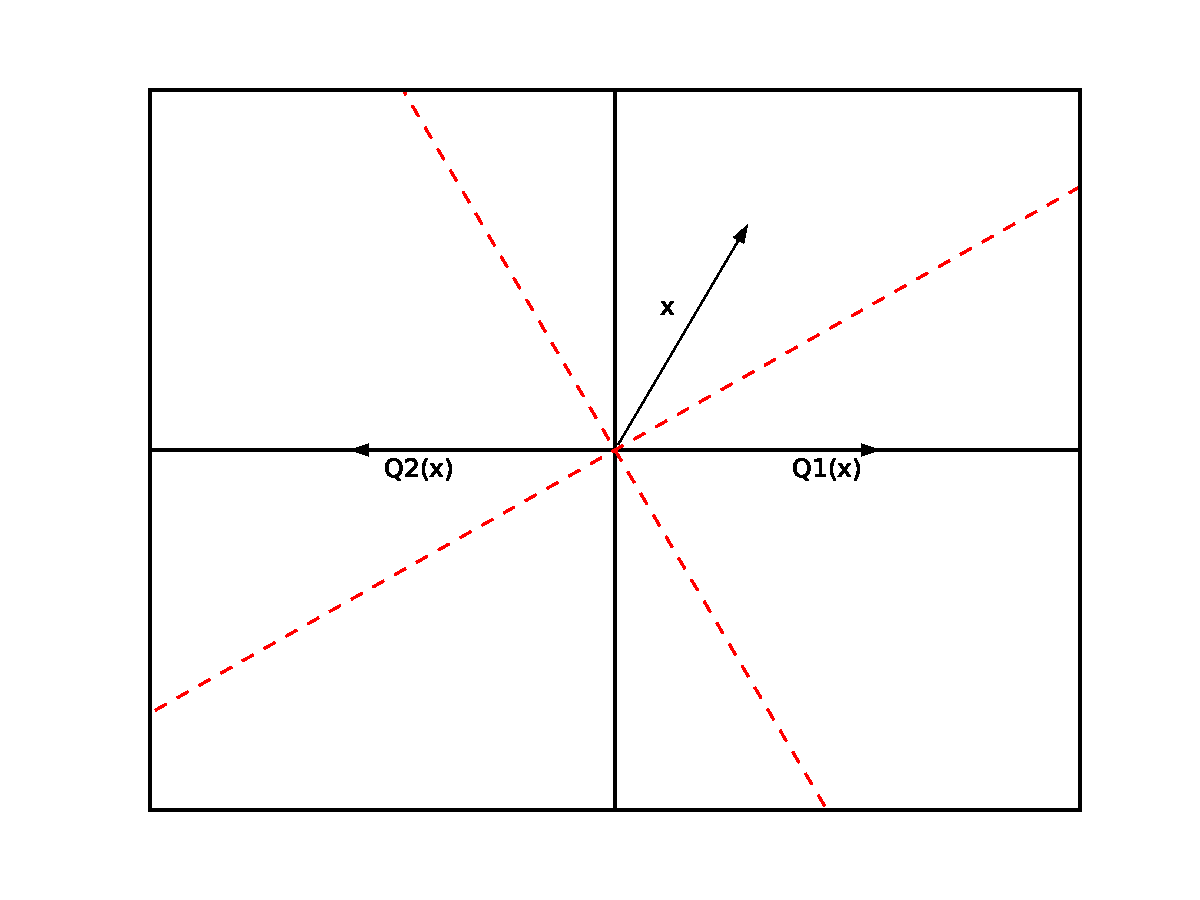
\includegraphics[width= \textwidth]{fig2}
\caption{two reflectors}
\label{fig:two reflectors}
\end{figure}

%TODO: explain notation, fix algorithm
\begin{algorithm}
\caption{Householder triangularization. This algorithm returns orthonormal $Q$ and upper triangular $R$ satisfying $A = QR$}
\label{Alg:Householder}
\begin{algorithmic}[1]
\Procedure{Householder}{$A$}
\State $m, n \gets \text{shape} \left( A \right)$
\State $R \gets \text{copy} \left( A \right)$
\State $Q \gets I_m$
\For{$0 \leq k < n-1$}
    \State $u_k \gets \text{copy} \left( R_{k:,k} \right)$
    \State $u_{k_0} \gets u_{k_0} + \text{sign} \left( u_{k_0} \right) \norm{u_k}$
    \State $u_k \gets u_k / \norm{u_k}$
    \State $R_{k:,k:} \gets R_{k:,k:} - 2 u_k \left( u_k^\mathsf{H} R_{k:,k:} \right)$
    \State $Q_{k:} \gets Q_{k:} - 2 u_k \left( u_k^\mathsf{H} Q_{k:} \right)$
\EndFor
\State \pseudoli{return} $Q^\mathsf{H}, R$
\EndProcedure
\end{algorithmic}
\end{algorithm}


\begin{problem}
\label{prob:HouseholderQR}
Write a function \li{householder} that accepts an array $A$ as input, and performs
the algorithm described above to compute the QR decomposition of $A$. Return the
matrices $Q$ and $R$.

It is simple to check that your code works: multiply the two output matrices
of your function, and check that the result matches the original input matrix.

Another important thing to notice is that an outer product is needed to compute $v_k \left( v_k^\mathsf{H} A[k:,k:] \right)$, not an inner product.
Make sure this is accounted for when you write the code to run this algorithm. You can either make the vectors $v_k$ column vectors (two dimensional with a single column) instead of just one-dimensional arrays, or you can use the built in function \li{np.outer} in the appropriate location.
\end{problem}

\begin{comment}
\subsection*{Stability of the Householder QR algorithm}
We will now examine the stability of the Householder QR algorithm.
We will use SciPy's built in QR factorization which uses Householder reflections internally.

Try the following.

\begin{lstlisting}
>>> Q, X = la.qr(np.random.rand(500,500)) # create a random orthonormal matrix:
>>> R = np.triu(np.random.rand(500,500)) # create a random upper triangular matrix
>>> A = np.dot(Q,R) # Q and R are the exact QR decomposition of A
>>> Q1, R1 = la.qr(A) # compute QR decomposition of A
\end{lstlisting}

Observe:

\begin{lstlisting}
>>> la.norm(Q1-Q)/la.norm(Q) # check error in Q
0.282842955725
>>> la.norm(R1-R)/la.norm(R) # check error in R
0.0428922016647
\end{lstlisting}

This is terrible!
This algorithm works in $16$ decimal points of precision, but $Q_1$ and $R_1$ are only accurate to $0$ and $1$ decimal points, respectively.
We've lost $16$ decimal points of precision!

Don't lose hope.
Check how close the product $Q_1 R_1$ is to $A$.
\begin{lstlisting}
>>> A1 = Q1.dot(R1)
>>> np.absolute(A1 - A).max()
3.9968028886505635e-15
\end{lstlisting}
We've now recovered $15$ digits of accuracy.
Considering the error relative to the norm of $A$ (using the 2-norm for matrices), we see that this relative error is even smaller.
\begin{lstlisting}
>>> la.norm(A1 - A, ord=2) / la.norm(A, ord=2)
8.8655568331889288e-16
\end{lstlisting}
The errors in $Q_1$ and $R_1$ were somehow ``correlated," so that they canceled out in the product.
The errors in $Q_1$ and $R_1$ are called \emph{forward errors}.
The error in $A_1$ is the \emph{backward error}.

In fact, the large errors in \li{Q1} and \li{R1} were not because the algorithm was bad, it was because $A$ was poorly conditioned.
The condition number for randomly generated upper triangular matrices is generally very high, and this was the case here.
This has, in turn, made the condition number of $A$ extremely large.

Try the following to compute the condition number of $A$.
In this case the condition number of $A$ and $R$ are computed to be different, though, in theory, they should be exactly the same.
\begin{lstlisting}
>>> from numpy.linalg import cond
>>> cond(A)
4.1426075832870472e+18
>>> cond(R)
3.1767577244363792e+19
\end{lstlisting}

Householder QR factorization is more numerically stable than Gram-Schmidt or even Modified Gram-Schmidt (MGS).
However, MGS is still useful for some types of iterative methods because it finds the orthonormal basis one vector at a time instead of all at once (for an example see Lab \ref{lab:EigSolve}).
\end{comment}

\subsection*{Upper Hessenberg Form}
An upper Hessenberg matrix is a square matrix with zeros below the first subdiagonal.
Every  $n \times n$ matrix $A$ can be written $A = Q^THQ$ where $Q$ is orthonormal and $H$ is an upper Hessenberg matrix, called the Hessenberg form of $A$.

A fast algorithm for computing the QR decomposition of a Hessenberg matrix will be taught in Lab \ref{lab:givens}. This algorithm in turn leads to a fast algorithm for finding eigenvalues of a matrix, which will be discussed in Lab \ref{lab:EigSolve}.

For now, we will outline an algorithm for computing the upper Hessenberg form of any matrix. 
Like Householder triangularization, this algorithm uses Householder transformations.
To find orthogonal $Q$ and upper Hessenberg $H$ such that $A = Q^THQ$, it suffices to find such matrices that satisfy $Q^TAQ=H$. 
Thus, our strategy is to multiply $A$ on the right and left by a series of orthonormal matrices until it is in Hessenberg form.
If we use the same $Q_1$ as in the first step of the Householder algorithm, then with $Q_1 A$ we introduce zeros in the first column of $A$.
However, since we now have to multiply $Q_1 A$ on the left by $Q_1^T$, all those zeros are destroyed.

Instead, let's try choosing a $Q_1$ that fixes $e_1$ and reflects the first column of $A$ into the span of $e_1$ and $e_2$. 
Because $Q_1$ fixes $e_1$, the product $Q_1A$ leaves the first row of $A$ alone, and $(Q_1A)Q_1^T$ leaves the first column of $(Q_1A)$ alone.
If $A$ is a $5 \times 5$ matrix, this looks like
\[
\begin{array}{ccccc}
\begin{pmatrix}
* & * & * & * & * \\
* & * & * & * & * \\
* & * & * & * & * \\
* & * & * & * & * \\
* & * & * & * & *
\end{pmatrix}
&\underrightarrow{Q_1 \cdot }&
\begin{pmatrix}
* & * & * & * & * \\
* & * & * & * & * \\
0 & * & * & * & * \\
0 & * & * & * & * \\
0 & * & * & * & *
\end{pmatrix}
&\underrightarrow{\cdot Q_1^T }&
\begin{pmatrix}
* & * & * & * & * \\
* & * & * & * & * \\
0 & * & * & * & * \\
0 & * & * & * & * \\
0 & * & * & * & *
\end{pmatrix}
\\
A & & Q_1A & & (Q_1 A) Q_1^T
  \end{array}
\]
We now iterate through the matrix until we obtain
\begin{equation*}
Q_3 Q_2 Q_1 A Q_1^T Q_2 ^T Q_3^T =
\begin{pmatrix}
* & * & * & * & * \\
* & * & * & * & * \\
0 & * & * & * & * \\
0 & 0 & * & * & * \\
0 & 0 & 0 & * & *
\end{pmatrix}.
\end{equation*}

When $A$ is Hermitian, its upper Hessenberg form is a tridiagonal matrix. 
This is because the $Q_i$'s zero out everything below the first subdiagonal of $A$ and the $Q_i^T$'s zero out everything above the first superdiagonal.
Thus, the Hessenberg form of a Hermitian matrix is especially useful, since as we saw in Lab \ref{lab:complexity}, tridiagonal matrices make computations fast.

The pseudocode for computing the Hessenberg form of a matrix is shown in Algorithm \ref{Alg:Hessenberg}.
Notice that this algorithm is very similar to Algorithm \ref{Alg:Householder}.

\begin{algorithm}
\caption{Reduction to Hessenberg Form}
\label{Alg:Hessenberg}
\begin{algorithmic}[1]
\Procedure{Hessenberg}{$A$}
\State $m, n \gets \text{shape}(A)$
\State $H \gets \text{copy}(A)$
\State $Q \gets I_m$
\For{$0 \leq k < n-2$}
    \State $u_k \gets H_{k+1:, k}$
    \State $u_{k_0} \gets u_{k_0} + \text{sign}(u_{k_0}) \norm{u_k}$
    \State $u_k \gets u_k/\norm{u_k}$
    \State $H_{k+1:,k:} \gets H_{k+1:,k:} - 2u_k(u_k^\mathsf{H} H_{k+1:,k:})$
    \State $H_{:,k+1:} \gets H_{:,k+1:} - 2(H_{:,k+1:} u_k) u_k^\mathsf{H}$
    \State $Q_{k+1:} \gets Q_{k+1:} - 2u_k(u_k^\mathsf{H} Q_{k+1:})$
\EndFor
\State \pseudoli{return} $Q, H$
\EndProcedure
\end{algorithmic}
\end{algorithm}

\begin{problem}
\label{prob:hessenberg}
Write a function \li{hessenberg} that computes the Hessenberg form of a real-valued
input matrix $A$. The function should return $Q$ and $H$ satisfying $A = Q^THQ$,
where $Q$ is orthonormal and $H$ has zeros below the first subdiagonal.

The code for this algorithm will be fairly similar to the code for the QR factorization using Householder reflections.
This factorization technique will be used later on in Lab \ref{lab:EigSolve}.
Notice what happens when you compute the Hessenberg factorization of a Hermitian matrix.
\end{problem}

%Sources: http://www.cs.unc.edu/~krishnas/eigen/node5.html
% http://en.wikipedia.org/wiki/Givens_rotation
%http://en.wikipedia.org/wiki/QR_decomposition
%	Note the Operation count: Householder is 2/3 n^3, MGS is 2 n^3
%http://en.wikipedia.org/wiki/QR_algorithm
%Applied Numerical methods using MATLAB by Yang has some code written for this
%http://www.math.kent.edu/~reichel/courses/intr.num.comp.2/lecture21/evmeth.pdf
%	These are eigenvalue algorithms explained carefully
%http://en.wikipedia.org/wiki/Householder_transformation
%Numerical Linear Algebra, by Lloyd N. Trefethen and David Bau III, Chapters 10 and 16 

